% !TEX root = main.tex

\section{多层神经网络} % 6.1-6.6 6.8 (6.9)
% 前馈网
% BP
% 误差表面
% Bayes与NN
% 激活函数
% 权重衰减, early stoping

三层神经网络:输入层、隐含层、输出层,也称多层感知器(multilayer perceptron, MLP)
\begin{figure}[H]
\centering
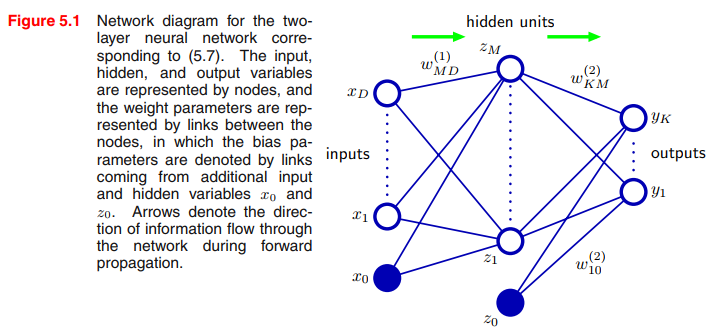
\includegraphics[width=0.8\linewidth]{fig/forward_propagation.png}
\end{figure}

前馈运算如下,判别函数$y_k(\vx,\vw)$为每个输出单元产生的信号
\[y_{k}(\mathbf{x}, \mathbf{w})=\sigma\left(\sum_{j=1}^{M} w_{k j}^{(2)} h\left(\sum_{i=1}^{D} w_{j i}^{(1)} x_{i}+w_{j 0}^{(1)}\right)+w_{k 0}^{(2)}\right)\]

任何从输入到输出的连续映射函数都可以用一个三层非线性网络实现,只要有足够的隐单元$M$、适当的非线性函数和权值。

最小化误差函数
\[E(\mathbf{w})=\frac{1}{2} \sum_{n=1}^{N}\left\|\mathbf{y}\left(\mathbf{x}_{n}, \mathbf{w}\right)-\mathbf{t}_{n}\right\|^{2}\]

隐含层到输出层的权重更新公式为
\[\Delta w_{kj}=\eta\delta_k y_j=\eta(t_k-z_k)f'(net_k)y_j\]
输入层到隐含层的权重更新公式为
\[\Delta w_{ji}=\eta x_i\delta_j=\eta\lrs{\sum_{k=1}^c w_{kj}\delta_k}f'(net_j)x_i\]

sigmoid函数
\[f(\text{net})=a\tanh(b\cdot\text{net})=a\lrs{\frac{1-\ee^{-b\cdot \text{net}}}{1+\ee^{-b\cdot\text{net}}}}=\frac{2a}{1+\ee^{-b\cdot\text{net}}}-a\]